\chapter{Técnicas auxiliares}
\section{Origen}
En los siguientes capítulos se habla de usar técnicas diferentes
para cada paso, con parámetros definidos y concretos. \\
La elección de estas técnicas junto con sus parámetros no se trata de
una elección arbitraria. Para llegar a la mejor solución, es decir, la
que encuentre los datos necesarios de forma exacta y sea genérica (que
sirva para todas las imágenes), se llevó a cabo un estudio del
funcionamiento y resultados de todas las posibles técnicas a aplicar.
Para ello se desarrollaron, en la mayoría de casos, algoritmos
auxiliares de visión computarizada que permitieran encontrar de forma
eficaz la técnica más adecuada en cada caso.

\section{Implementación}
Dado que el número de técnicas es muy amplio, así como los valores que
pueden tomar sus parámetros, se desarrollaron una serie de programas
destinados a probar las transformaciones aplicadas por dichas técnicas
de forma fácil. Para ello se generaron diversas interfaces gráficas
que, valiéndose de barras, permiten ver en tiempo real las
transformaciones aplicadas a una imagen para así poder compararlas y
encontrar la que mejores resultados proporcione. Además este tipo de
interfaces gráficas permitieron a los oftalmólogos interactuar y
comprender los resultados obtenidos, así como también de hacer
propuestas e indicaciones para realizar mejoras que de otra manera no
podrían haber hecho. \\

A continuación se muestra una serie de imágenes de ejemplo acerca del
uso de barras de interacción en tiempo real para reducir el tiempo de
estudio, facilitar la presentación de las técnicas y generar así una
mejor retroalimentación con los oftalmólogos.

\begin{figure}[H]
  \caption{Barras de interacción con \emph{thresholds}}
  \centering \setlength\fboxsep{0pt} \setlength\fboxrule{0.5pt}
  \fbox{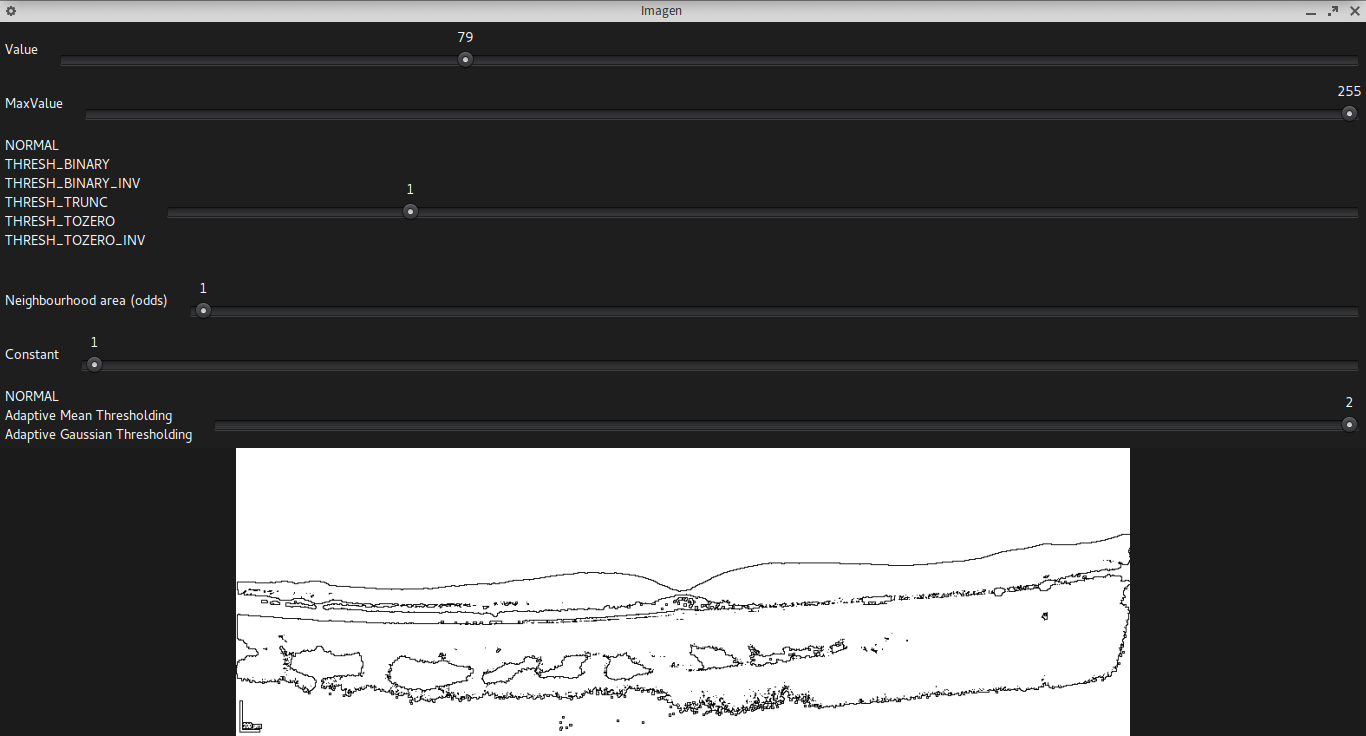
\includegraphics[width=\textwidth]{imagenes/tecnicas_aux/barrasThresholds.png}}
\end{figure}
\begin{figure}[H]
  \caption{Barras de interacción con \emph{Canny}}
  \centering \setlength\fboxsep{0pt} \setlength\fboxrule{0.5pt}
  \fbox{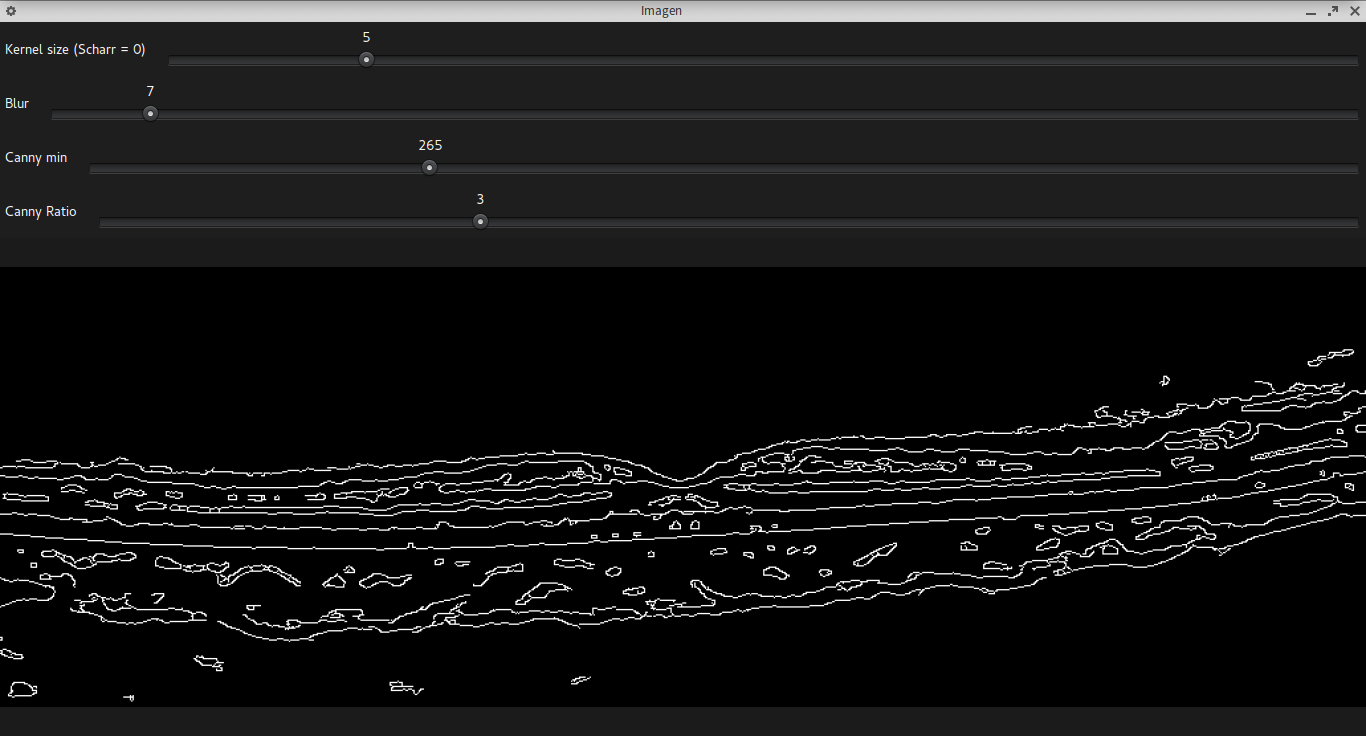
\includegraphics[width=\textwidth]{imagenes/tecnicas_aux/barrasCanny.png}}
\end{figure}

Ejemplo de comunicación entre la bibliotecas \emph{OpenCV} para
generar las barras de interacción y \emph{SimpleCV} para la detección
de los \emph{blobs}.

\begin{figure}[H]
  \caption{Barras de interacción para detección de \emph{blobs}}
  \centering \setlength\fboxsep{0pt} \setlength\fboxrule{0.5pt}
  \fbox{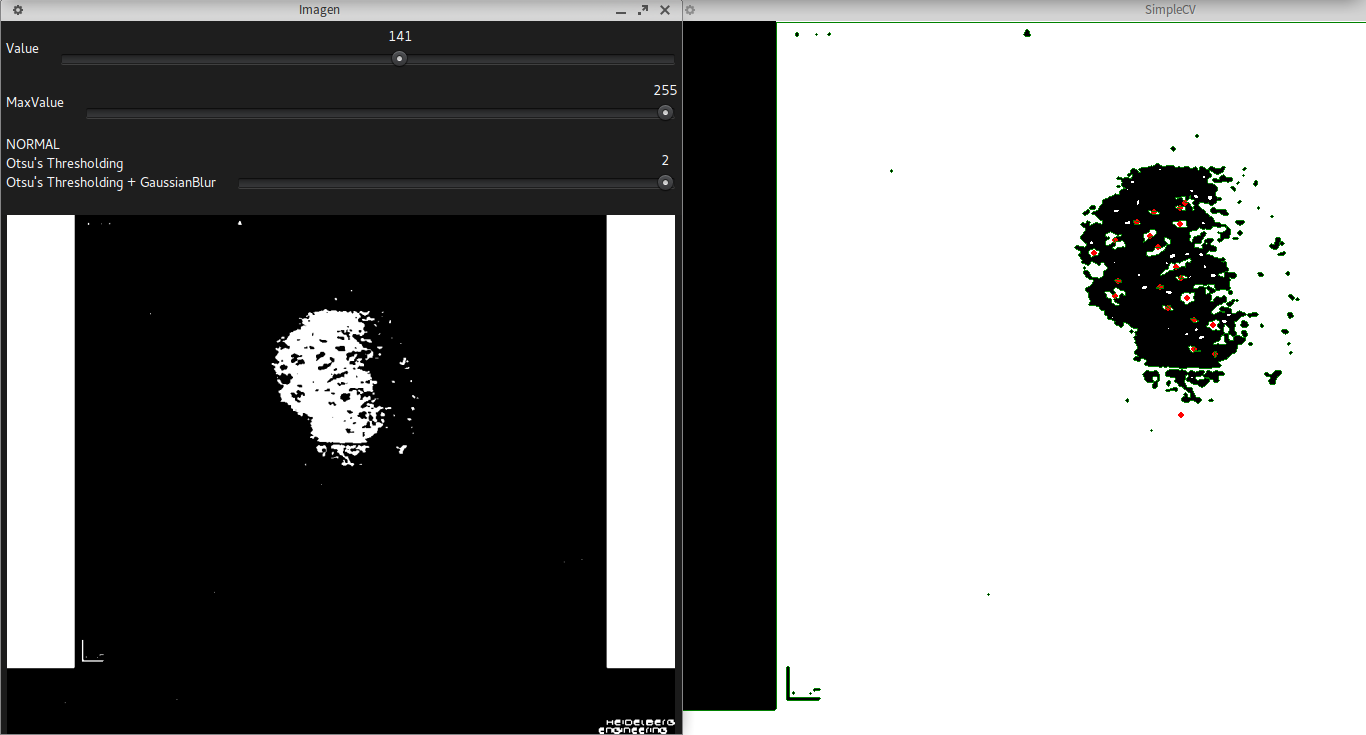
\includegraphics[width=\textwidth]{imagenes/tecnicas_aux/barrasInteraccion.png}}
\end{figure}
